\chapter{Custos: A First-Generation SSaaS Prototype}
\label{chap:custos}

Custos\footnote{Custos is Latin for ``guard''.} is a prototype SSP
server, SSaaS protocol, and SSaaS client ecosystem used to demonstrate
and explore SSaaS concepts. Custos is optimized for cryptographic key
storage, making it primarily a Key Storage as a Service (KSaaS)
implementation. The chapter provides an overview of Custos and some of
its design insights. Additional information is available at
\cite{custos-masters} and \cite{custos-trios}.

\section{Architecture}
\label{chap:custos:arch}

\begin{figure}[t]
  \centering
  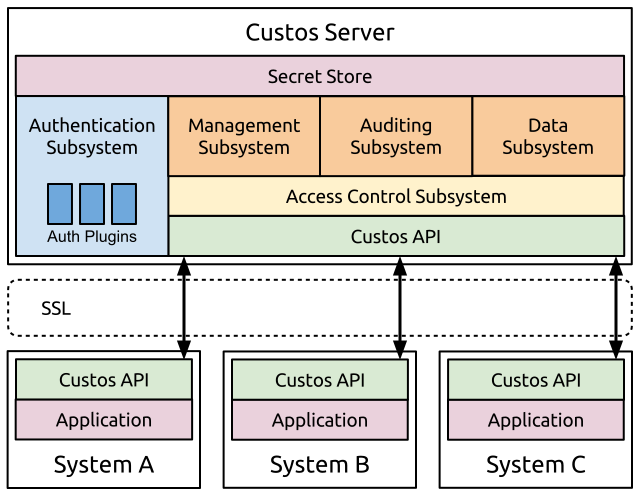
\includegraphics[height=200px]{./figs/out/Custos-Overview.pdf}
  \caption{Custos's Architecture}
  \label{fig:custos-overview}
\end{figure}

Figure \ref{fig:custos-overview} shows the core Custos components. The
bulk of Custos's functionality is handled on the SSP server. The
Custos SSP server implements the following components:

\begin{packed_desc}
\item[API:] Handles all Custos requests, including requests for
  key:value objects, requests for audit data, and requests to modify
  access control parameters. The API is designed to promote a variety
  of Custos-compliant server implementations.
\item[Access Control:] Compares the set of provided authentication
  attributes (calling into the authentication system to verify them)
  to the set of required authentication attributes to determine if a
  Custos request should be allowed or denied.
\item[Authentication:] Verifies the validity of any authentication
  attributes associated with a given Custos request via a pluggable
  authentication module interface capable of supporting a variety of
  authentication primitives.
\item[Data:] Handles data requests (e.g. get, set, create, and
  delete of key:value objects).
\item[Auditing:] Handles audit requests and logs all Custos
  requests.
\item[Management:] Handles management requests (e.g. the
  manipulating access control parameters).
\item[Key-Value Secret Store:] Stores persistent data such as end user
  secrets (e.g. encryption keys) as well as internal state
  (e.g. access control requirements).
\end{packed_desc}

\subsection{Access Control}
\label{chap:custos:arch:ac}

Custos employs a unique access control scheme called Access Control
Chains (ACCs). In this scheme each Custos permission (e.g. reading a
specific secret) is associated with one or more Access Control
Chains. Each Access Control chain consists of an ordered list of
Authentication Attributes (AA). Each Authentication Attribute
represents a single authentication primitive (e.g. supplying the
correct password, or verifying one's identity via a cryptographic
authentication certificate). In order to gain a specific permissions
in Custos, a user must be able to satisfy all AAs in at least one of
the permission's associated ACCs. This scheme enables highly flexible
access control semantics, allowing Custos secrets to be stored for a
variety of applications.

\begin{figure}[t]
  \centering
  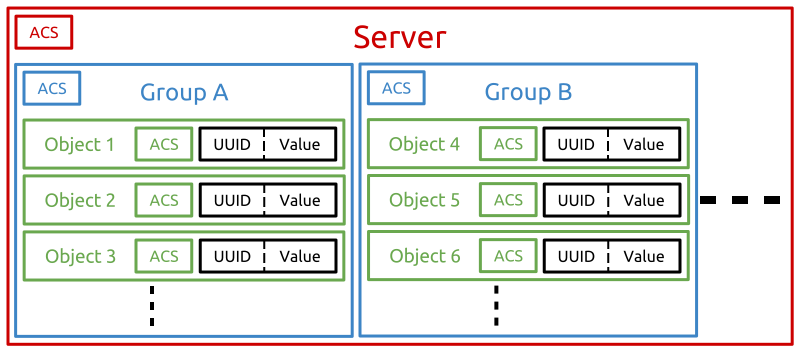
\includegraphics[height=200px]{./figs/out/Custos-OU.pdf}
  \caption{Custos's Organizational Units}
  \label{fig:custos-ou}
\end{figure}

In order to discuss the Custos access control system, it is necessary
to explain the Custos \emph{organizational units} (OUs): the core
Custos data structures. The Custos architecture specifies three
organizational units (Figure~\ref{fig:custos-ou}): a server, a group,
and a key:value object. The server unit is used to specify server-wide
configuration. A server has one or more groups associated with it. A
group is used to slice a server between a variety of administrative
domains (e.g. separate customers). A group, in turn, has an arbitrary
number of key:value objects associated with it. Each OU is responsible
for the creation of OU instances beneath it: i.e. servers create
groups and groups create objects.

\begin{figure}[t]
  \centering
  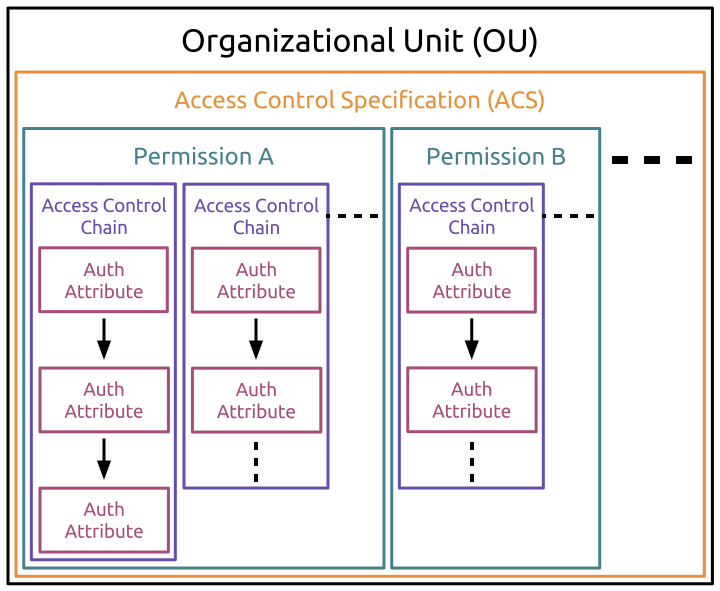
\includegraphics[height=200px]{./figs/out/Custos-ACS.pdf}
  \caption{Access Control Specification Components}
  \label{fig:custos-acs}
\end{figure}

The Custos access control abstraction revolves around designating an
\emph{Access Control Specification} (ACS) for each OU in the Custos
architecture. An ACS consists of three components
(Figure~\ref{fig:custos-acs}). Each ACS contains a full list of the
applicable \emph{permissions} for the given OU. Associated with each
permission is one or more \emph{access control chains} (ACCs). Each
ACC consists of an ordered list of \emph{authentication attributes}.

\subsubsection{Permissions}
\label{chap:custos:arch:ac:perms}

\begin{table}[!thb]
  \footnotesize
  \centering
  \tabulinesep = 2pt
  \begin{tabu} to \textwidth
    { | X[1.25,l,m]
      | X[.5,l,m]
      | X[4,l,m]
      | }
    \hline
    \textbf{Permission}
    & \textbf{OU}
    & \textbf{Rights}
    \\ \hline
    \texttt{srv\_grp\_create}
    & Server
    & create groups on a Custos server
    \\ \hline
    \texttt{srv\_grp\_list}
    & Server
    & list groups on a Custos server
    \\ \hline
    \texttt{srv\_grp\_override}
    & Server
    & escalate to any group-level permission, overriding the per-group ACS
    \\ \hline
    \texttt{srv\_audit}
    & Server
    & read all server-level audit information
    \\ \hline
    \texttt{srv\_clean}
    & Server
    & delete all server-level audit information
    \\ \hline
    \texttt{srv\_acs\_get}
    & Server
    & view the server-level ACS controlling the permissions in this list
    \\ \hline
    \texttt{srv\_acs\_set}
    & Server
    & update the server-level ACS controlling the permissions in this list
    \\ \hline
    \texttt{grp\_obj\_create}
    & Group
    & create a key:value objects within the given group
    \\ \hline
    \texttt{grp\_obj\_list}
    & Group
    & list key:value objects within the given group
    \\ \hline
    \texttt{grp\_obj\_override}
    & Group
    & escalate to any object-level permission, overriding the per-object ACS
    \\ \hline
    \texttt{grp\_delete}
    & Group
    & delete the given group on a Custos server
    \\ \hline
    \texttt{grp\_audit}
    & Group
    & read all group-level audit information
    \\ \hline
    \texttt{grp\_clean}
    & Group
    & delete all group-level audit information
    \\ \hline
    \texttt{grp\_acs\_get}
    & Group
    & view the group-level ACS controlling the permissions in this list
    \\ \hline
    \texttt{grp\_acs\_set}
    & Group
    & update the group-level ACS controlling the permissions in this list
    \\ \hline
    \texttt{obj\_delete}
    & Object
    & delete the given key:value object within the given group
    \\ \hline
    \texttt{obj\_read}
    & Object
    & read the given key:value object within the given group
    \\ \hline
    \texttt{obj\_update}
    & Object
    & create a new version of the given key:value object within the given group
    \\ \hline
    \texttt{obj\_audit}
    & Object
    & read all object-level audit information
    \\ \hline
    \texttt{obj\_clean}
    & Object
    & delete all object-level audit information
    \\ \hline
    \texttt{obj\_acs\_get}
    & Object
    & view the object-level ACS controlling the permissions in this list
    \\ \hline
    \texttt{obj\_acs\_set}
    & Object
    & update the object-level ACS controlling the permissions in this list
    \\ \hline
  \end{tabu}
  \caption{Custos Permissions}
  \label{tab:custos-permissions}
\end{table}

Each Custos ACS contains a list of permissions: rights to perform
specific Custos actions. Custos defines permissions for each OU:
i.e. per-server permissions, per-group permissions, and per-object
permissions (Table~\ref{tab:custos-permissions}).  Unlike many access
control systems, Custos has no notion of object ownership. Instead, it
relies on explicitly granting each right an owner would traditionally
hold via explicit permissioning. Custos permissions are initially set
when the associated OU is created. After creation, each ACS can be
updated by anyone granted the necessary \texttt{acs\_set} permission
for the specific OU instance. Custos group and server ACSs also
includes an ``override'' permission. This permission can be used to
override the permissions of a lower-level OU's ACS. For example,
anyone gaining the \texttt{srv\_grp\_override} permission can use it
to gain any of the rights normally granted via a group-level
permission. Likewise, anyone gaining the \texttt{grp\_obj\_override}
permission can use it to gain any of the rights normally granted via
an object-level permission. These overrides exist for administrative
tasks: allowing server admins to manipulate group data, and allowing
group admins to manipulate object data.

\subsubsection{Access Control Chains}
\label{chap:custos:arch:ac:acc}

Each ACS permission has one or more associated access control chains
(ACCs). An access control chain is an ordered list of authentication
attributes (discussed in \S~\ref{chap:custos:arch:ac:aa}). In order for a
request to be granted a specific permission, it must be able to
provide authentication attributes satisfying at least one of the ACCs
associated with that permission. If a user wishes to disable access to
a permission, they can do so by associating the null ACC with that
permission. If the user wants to provide unrestricted access to a
permission, they may do so by associating an empty ACC with the
permission. For example, consider a key:value object whose
\texttt{obj\_read} permission has the following ACC set:

\begin{Verbatim}[samepage=true, fontsize=\footnotesize]
[ (user_id = Andy),
  (ip_src = 192.168.1.0/24),
  (psk = 12345) ]
[ (user_id = Andy),
  (ip_src = 192.168.1.0/24),
  (cert_id = 0x32C59C00) ]
[ (user_id = John),
  (psk = Swordfish) ]
\end{Verbatim}

In order for a read request for the associated key:value object to
succeed, the user would have to make sure that their request contained
all the authentication attributes in at least one of the lists
above. In the case of the first ACC, that would mean attaching the
'user\_id' attribute with a value of 'Andy', as well as attaching the
'psk' attribute with a value of '12345'. The 'ip\_src' attribute is an
implicit attribute (see \S~\ref{chap:custos:arch:ac:aa}) and will be
automatically appended to our request when received by the Custos
server. In order to satisfy it, the user must send their request from
the 192.168.1.0 subnet. In the case of the second ACC, the user still
needs the 'Andy' username and must satisfy the IP restriction, but
this time they must also prove that they have access to the private
key associated with the specified authentication certificate instead
of providing a password. The third ACC grants access to an additional
user, John, with his own password. As long as a user can satisfy at
least one ACC in a set of ACCs for a given permission, they are
granted the right to perform actions associated with the permission.

This system is highly flexible. Take, for example, the lack of
explicit username support anywhere in the Custos specification. As was
done above, usernames simply become another authentication
attribute. Often a username will be the first attribute in a ACC to
allow for all following attributes to be specified relative to a given
username (as shown in the example above). But there's nothing special
about usernames. An administrator could just have easily started each
ACC with an IP attribute, requiring a separate password based upon the
location a user is making their request from. The combination of
simple ordered attribute lists and a wide range of flexible attributes
makes for powerful access control semantics.

Another point worth noting is that sets of ACCs can be converted into
ACC trees, often simplifying the understanding or verification of
their semantic intent. ACC lists are converted into ACC trees by
combining common attributes across multiple ACC lists into single
nodes in an ACC tree. For example, the first two ACCs in the previous
set of ACCs could also be represented as:

\begin{center}
  \begin{tikzpicture}
    \tikzset{level distance=20pt}
    \tikzset{sibling distance=0pt}
    \Tree [
      .\texttt{\footnotesize (user\_id = Andy)}
      [
        .\texttt{\footnotesize (ip\_src = 192.168.1.0/24)}
        \texttt{\footnotesize (psk = 12345)}
        \texttt{\footnotesize (cert\_id = 0x32C59C00)}
      ]
    ]
  \end{tikzpicture}
\end{center}

Finally, where desired~\footnote{Custos's attribute prompting feature
  is a form of information leakage, so its use, and the associated
  trade-offs, are optional.}, the Custos API can continue to prompt
the user for the next N missing attribute types in a chain. When in
use, this feature allows a Custos server to engage in a back-and-forth
message exchange with a client to prompt the client through all
required attribute types in an ACC. For example, in the case where N
is equal to 1 and the previously mentioned ACCs are in effect, the
following set of transactions would occur:

\begin{packed_enum}
\item The user sends a read request with no attributes
\item The server respond that a username is required
\item The user resubmits the request with an attached username
  attribute equal to 'Andy'
\item The server responds that a password or a certificate is required
  (the IP attribute is implicit and is thus not prompted for)
\item The user resubmits the response with a password equal to '12345'
\item As long as the user's request originates from the specified IP
  range, the server will grant the request.
\end{packed_enum}

\subsubsection{Authentication Attributes}
\label{chap:custos:arch:ac:aa}

\begin{table}[thb]
  \footnotesize
  \centering
  \tabulinesep = 2pt
  \begin{tabu} to \textwidth
    { | X[1.5,l,m]
      | X[1,l,m]
      | X[3,l,m]
      | }
    \hline
    \textbf{Type}
    & \textbf{Class}
    & \textbf{Description}
    \\ \hline
    \texttt{ip\_src}
    & implicit
    & Request source IP
    \\ \hline
    \texttt{time\_utc}
    & implicit
    & Request arrival time
    \\ \hline
    \texttt{user\_id}
    & explicit
    & Arbitrary user ID
    \\ \hline
    \texttt{psk}
    & explicit
    & Arbitrary pre-shared key
    \\ \hline
  \end{tabu}
  \caption{Example Authentication Attributes}
  \label{tab:custos-attributes}
\end{table}

Each Access Control Chain contains one or more Authentication
Attributes (AAs). An authentication attribute is a generic container
for authentication data. AAs contain the following information:

\begin{packed_desc}
\item[Class] The top level classification property of an AA. It is
  used to designate the nature of a given AA. Currently, Custos
  specifies two possible values for class: ``implicit'' and
  ``explicit''. Implicit attributes are those that are automatically
  associated with a request (like an IP address). Explicit attributes
  are those that the user provides directly to Custos (like a
  username).
\item[Type] Within a given class, the AA type specifies which
  authentication plugin should handle a specific attribute.
\item[Value] The value contains the arbitrary data associated with a
  given attribute.
\end{packed_desc}

The Custos specification supports a flexible set of authentication
types. Each AA is processed by a specific AA plugin module allowing
for extensible authentication primitive support similar to systems
like PAM~\cite{samar1996}. Examples of potential Custos AA types are
shown in Table~\ref{tab:custos-attributes}.

\subsection{Protocol}

Custos employs a JSON-based RESTful HTTPS protocol for client-server
communication. The protocol exposes endpoints for secret management
(e.g. create, list, read, delete), access control (e.g. adding,
removing, and modifying access control rules), and auditing
(e.g. reading or clearing secret access history). Custos allows
arbitrary cryptographic key data to be associated with each ID for
secret storage purposes. Each ID:secret pair in Custos is associated
with a specific group. These groups can be used to allow multiple
users to administer a set of secrets and to control who can create new
secrets within a group.

The Custos API is secured via TLS/HTTPS. Custos servers are
authenticated over TLS via the standard public key infrastructure
(PKI) mechanisms (e.g. certificate authorities, etc)\footnote{In
  situations were the traditional PKI mechanisms are deemed
  undesirable, it may be possible to authenticate Custos servers via
  self-certifying mechanisms~\cite{ellison1996, mazieres1999}.}. API
requests are made to specific server HTTPS endpoints. The standard
HTTP verbs (\texttt{GET}, \texttt{PUT}, \texttt{POST}, and
\texttt{DELETE}) are used to multiplex related operations atop a
specific endpoint. Each combination of endpoint and verb defines a
specific API method. Each method requires a specific permission to
complete. All API message formats are composed in JSON. Binary data is
encoded as Base64 ASCII text. Authentication attributes are passed via
query string as URL-encoded JSON. Custos uses UUIDs~\cite{leach2005}
as keys, each associated with an arbitrary object for values. The full
API specification, including detailed message formats, example
messages, and a list of API methods and endpoints
see~\cite{custos-masters}.

In the Custos protocol, the server is completely agnostic to the
secret cryptographic keys it stores. Thus, a user may shard their
secret keys across multiple providers/servers if they wish. Because of
this fact, however, users must still manually set the appropriate ACCs
for a given secret across all Custos servers holding a share of that
secret. Likewise, a user must manually query each server holding a
share of a secret for audit data in order to aggregate the full audit
history for a given secret. Developing methods for more easily
coordinating the storage and management of a set of secret shares
across multiple SSPs is one of the focuses of the Tutamen design
discussed in Chapter~\ref{chap:tutamen}.

\section{Implementation}

Prototype implementations of both a Custos server and a sample Custos
client were created to to test and demonstrate the basic SSaaS
concepts proposed in this document. These implementation are described
below.

\subsection{SSP Server}

The Custos SSP server~\cite{custos-repo-server} is implemented in
Python. It is designed to use file-system backed key-value stores for
secret storage. The bulk of the Custos server code base is involved
with implementing the verification process for Access Control Chains
and the associated Access Attribute modules. The server leverages the
Flask~\cite{python-flask} web framework to implement the Custos API,
and provides HTTPS support via the Apache~\cite{apache} web server.
The server is capable of handling a few hundreds key requests per
second, depending on the complexity of the associated ACCs.

\subsection{EncFS}

\texttt{EncFS} is a sample SSaaS client~\cite{custos-repo-encfs}
created test the Custos SSP server and demonstrate an SSaaS-aware
application. \texttt{EncFS} implements a FUSE-based~\cite{fuse}
layered file system that provides transparent client side-encryption
atop an underlying file store. \texttt{EncFS} offloads its key storage
duties to the Custos SSP Server using the Custos SSaaS protocol. It
accomplishes this via \texttt{libcustos}, a C-library implementation
of the Custos protocol~\cite{custos-repo-libcustos}.

\texttt{EncFS}'s utilization of the SSaaS model allows it to support
many cloud-based use cases not readily supported by traditional
encrypted file-systems, all while minimizing the trust placed in
cloud-based storage providers and Custos SSPs. For example, when
mounted atop a Dropbox-backed directory, \texttt{EncFS} allows a user
to ensure that Dropbox has no access to the plain-text contents of a
user's files. None the less, users can still use Dropbox to sync a
file across multiple devices or share it with other users. The user
must simply update the access control attributes for a given file's
encryption key stored via their Custos SSP to allow access from other
user-owned devices or by other collaborating users. \texttt{EncFS}
accomplishes this without any need to modify Dropbox's storage
interface or otherwise change the manner is which existing cloud file
stores operate.

Adding the SSP encryption key request operation to the file read
process does incur an additional ~10 to ~100 milliseconds of latency
on file reads, primarily dependent on the network latency between the
client and the SSP~\cite{custos-trios}. None the less, it's unlikely
that most users will notice this additional latency in normal
day-to-day use (e.g. editing a text file, playing a media file,
viewing a photo, etc). This latency is also no worse then most
existing distributed or networked file system protocols would incur,
and in situations where an SSaaS client like \texttt{EncFS} is used in
conjunction with a distributed or networked file system, secret-access
operations can be performed in parallel with encrypted data-access
operations, ensuring that the SSP latency is not incurred in addition
to existing networked file system latency.

%%  LocalWords:  Custos SSaaS SSP Custos's ACCs AAs OUs OU ACS ACC ip
%%  LocalWords:  srv grp acs ACSs OU's src psk subnet utc HTTPS SSPs
%%  LocalWords:  EncFS libcustos KSaaS Tutamen
